En esta sección mostraremos un pequeño manual de uso del mod creado para \cities, así como su instalación.

\section{Instalación}

Para proceder a instalar el mod, necesitaremos una cuenta de \href{https://store.steampowered.com/}{Steam}. Una vez creada, y habiendo comprado e instalado \cities en Steam, vamos a la WorkShop de \cities y buscamos \textit{IndustryLP}. Deberíamos de encontrar una entrada al mod que aparece en la Figura \ref{fig:mod}. \\

\begin{figure}[h]
	\centering
	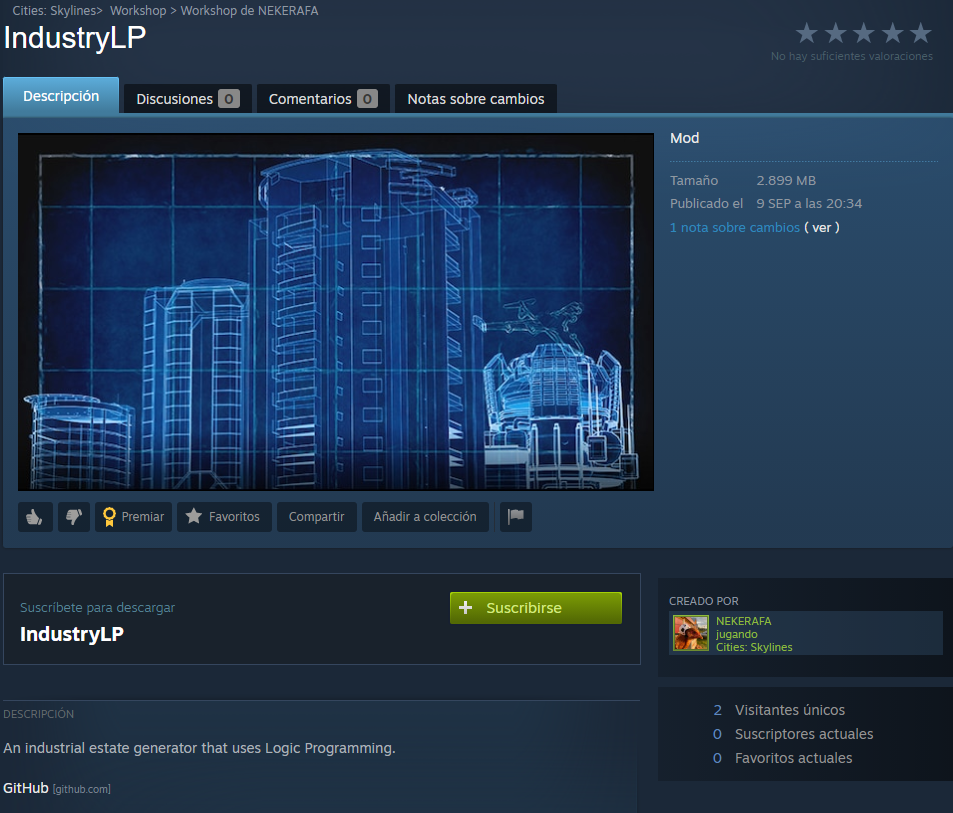
\includegraphics[width=\textwidth]{images/workshop}
	\caption{Página web del IndustryLP en la WorkShop de \cities.}
	\label{fig:mod}
\end{figure}

Una vez en la web del mod, solo tenemos que pulsar en el botón \texttt{Subscribe} para que la aplicación de escritorio instale los archivos necesario para ejecutar el mod.

\section{Uso}

Una vez subscritos, podemos ejecutar \cities. Para habilitar el mod, tenemos que entrar en el menú \texttt{Content Manager}, e ir a la sección \texttt{Mods}. Allí podremos buscar \textit{IndustryLP} y activarlo seleccionando el checkbox con la etiqueta \texttt{On / Off}, tal y como se muestra en la Figura \ref{fig:options}. \\

\begin{figure}[h]
	\centering
	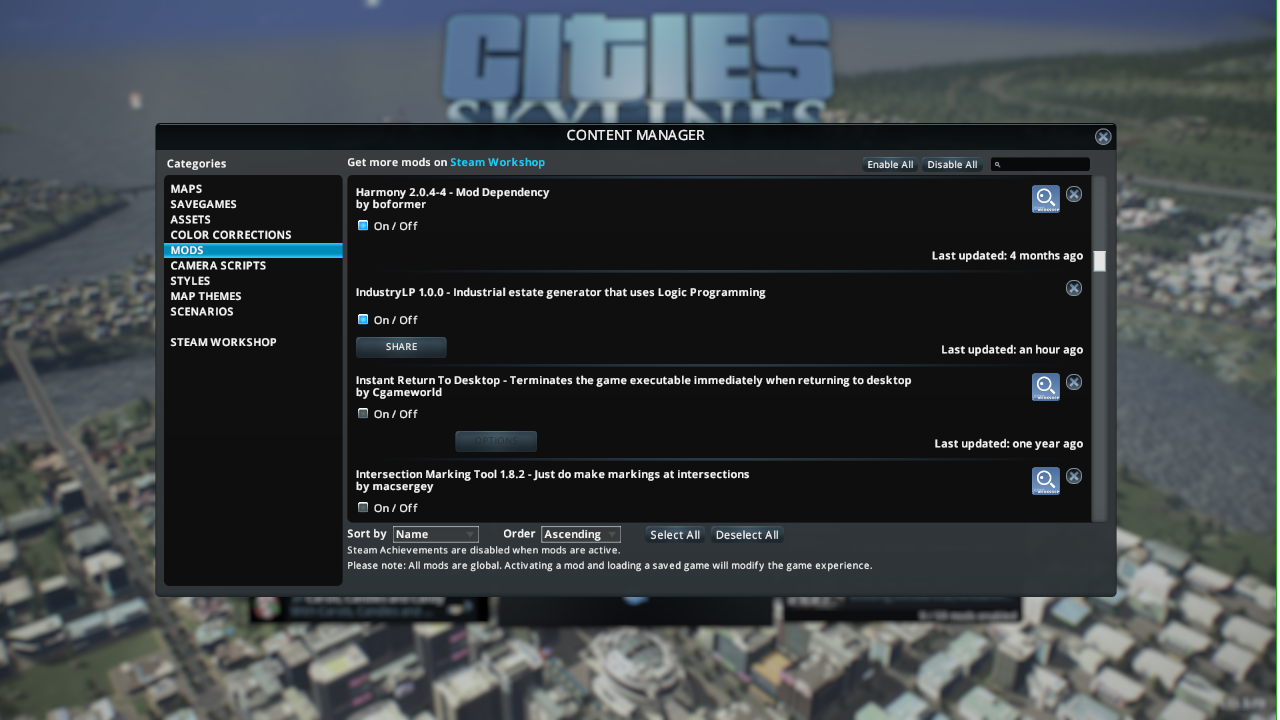
\includegraphics[width=\textwidth]{images/options}
	\caption{Activación de IndustryLP en \cities.}
	\label{fig:options}
\end{figure}

Con el mod activado, podemos empezar una nueva partida. Se nos activará un nuevo icono que permitirá lanzar el menú de la Figura \ref{fig:tool}. En el destacamos varias cosas:

\begin{figure}[h]
	\centering
	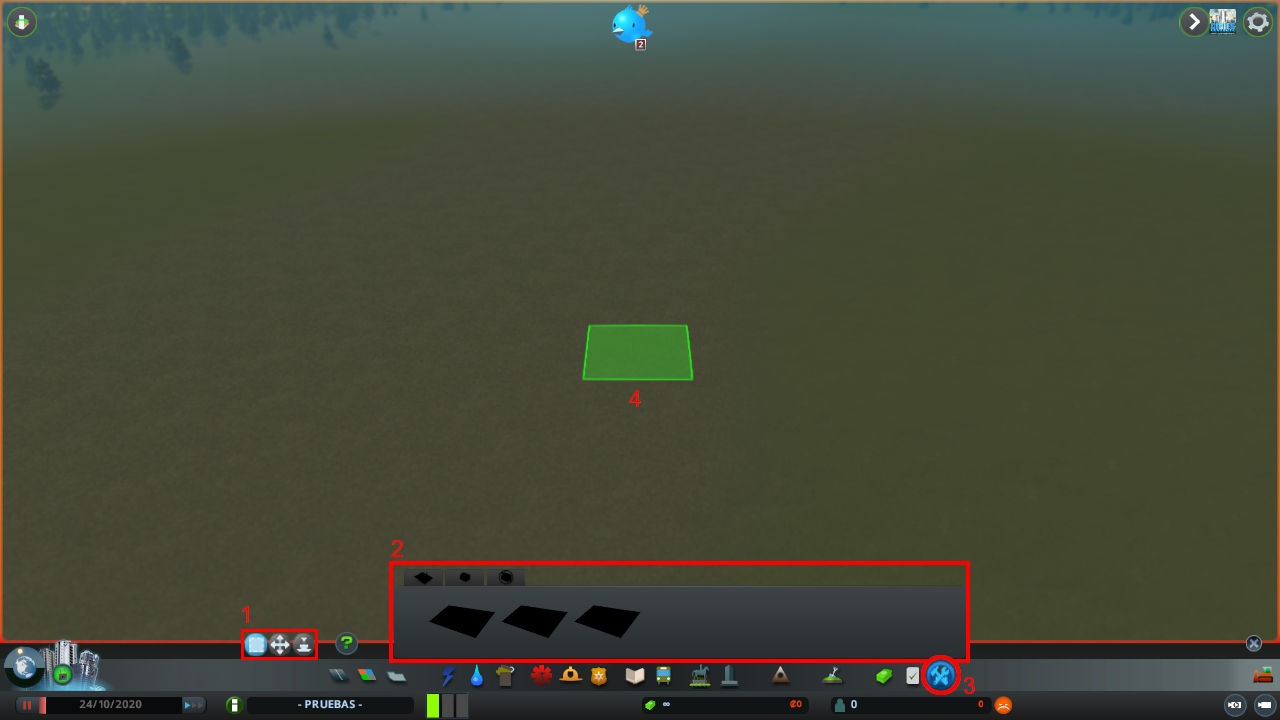
\includegraphics[width=\textwidth]{images/tool}
	\caption{Interfaz de IndustryLP.}
	\label{fig:tool}
\end{figure}

\begin{enumerate}
    \item \textbf{Acciones de la herramienta:} Se muestran tres iconos: Definir región, mover región y generar soluciones.
    \item \textbf{Panel de opciones:} En el podremos elegir las distribuciones predefinidas, así como definir preferencias y restricciones de edificios.
    \item Icono principal del mod.
    \item Cursor.
\end{enumerate}

\subsection{Definir región}

Cuando pulsamos en el icono de la acción \textbf{Definir región} se nos activará un cursor con un cuadrado verde en el mapa. Si mantenemos pulsado en una región, este cuadrado cambiará a una selección de color naranja. \\

Una vez terminada la selección, se nos mostrará la selección de color blanco, con cuatro puntos verdes en cada arista y uno en el centro, tal y como se muestra en la Figura \ref{fig:selection}. Si el tamaño no fuera el suficiente, esta selección será roja, y al dejar de pulsar se desmarcará al no ser válida, como recogemos en la Figura \ref{fig:bad-selection}.

\begin{figure}[h]
	\centering
	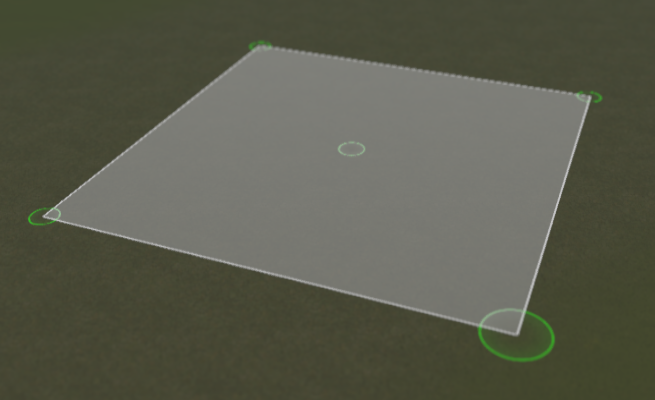
\includegraphics[width=0.5\textwidth]{images/selection}
	\caption{Región correctamente seleccionada.}
	\label{fig:selection}
\end{figure}

\begin{figure}[h]
	\centering
	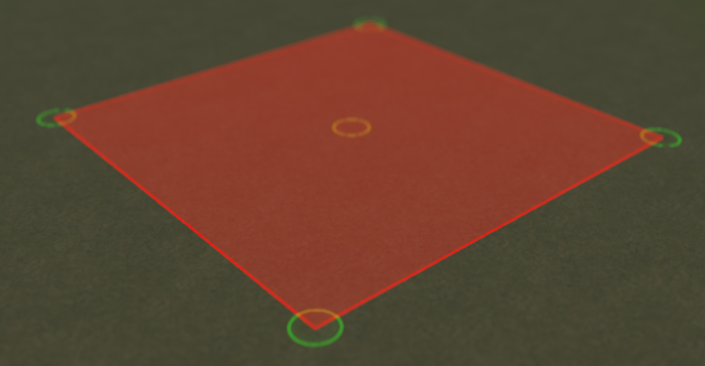
\includegraphics[width=0.5\textwidth]{images/bad-selection}
	\caption{Región con tamaño insuficiente.}
	\label{fig:bad-selection}
\end{figure}

\subsection{Mover región}

Una vez realizada una selección, se nos habilitará la acción de \textbf{Mover región} que nos mostrará la selección de la misma forma que en la Figura \ref{fig:selection}. \\

Esta acción nos permitirá modificar el la posición de cada uno de sus vértices verdes, así como mover la selección pulsando en el círculo central de la selección, y rotarla. Para rotarla tendremos que pulsar el botón derecho del ratón en cualquier parte del mapa, y sin soltarlo, moverlo.

\subsection{Distribuciones del terreno}

Cuando tengamos una selección hecha, se nos habilitará en el panel de opciones la pestaña de \textit{Distribuciones} (Figura \ref{fig:distributions-panel}). Al pinchar en cualquiera de las opciones, IndustryLP calculará que distribución hacer dentro de la selección. Este proceso puede tardar escasos segundos, los suficientes para que \cities se congele si la selección es muy grande.

\begin{figure}[h]
	\centering
	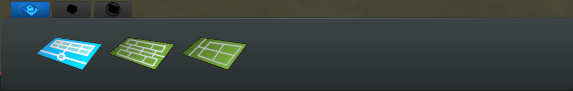
\includegraphics[width=\textwidth]{images/distributions}
	\caption{Panel con la lista de distribuciones.}
	\label{fig:distributions-panel}
\end{figure}

\subsection{Añadir preferencias / restricciones}

Con la distribución de caminos generada, se nos habilitará las pestañas de \textit{Preferencias} y \textit{Restricciones}, tal y como se muestra en la Figura \ref{fig:preferences}. En ellas, podremos seleccionar un edificio de industria que viene incluido en \cities y, o indicar su posición en el caso de una preferencia, o indicar a IndustryLP que no genere ese edificio en una posición dada. \\

\begin{figure}[h]
	\centering
	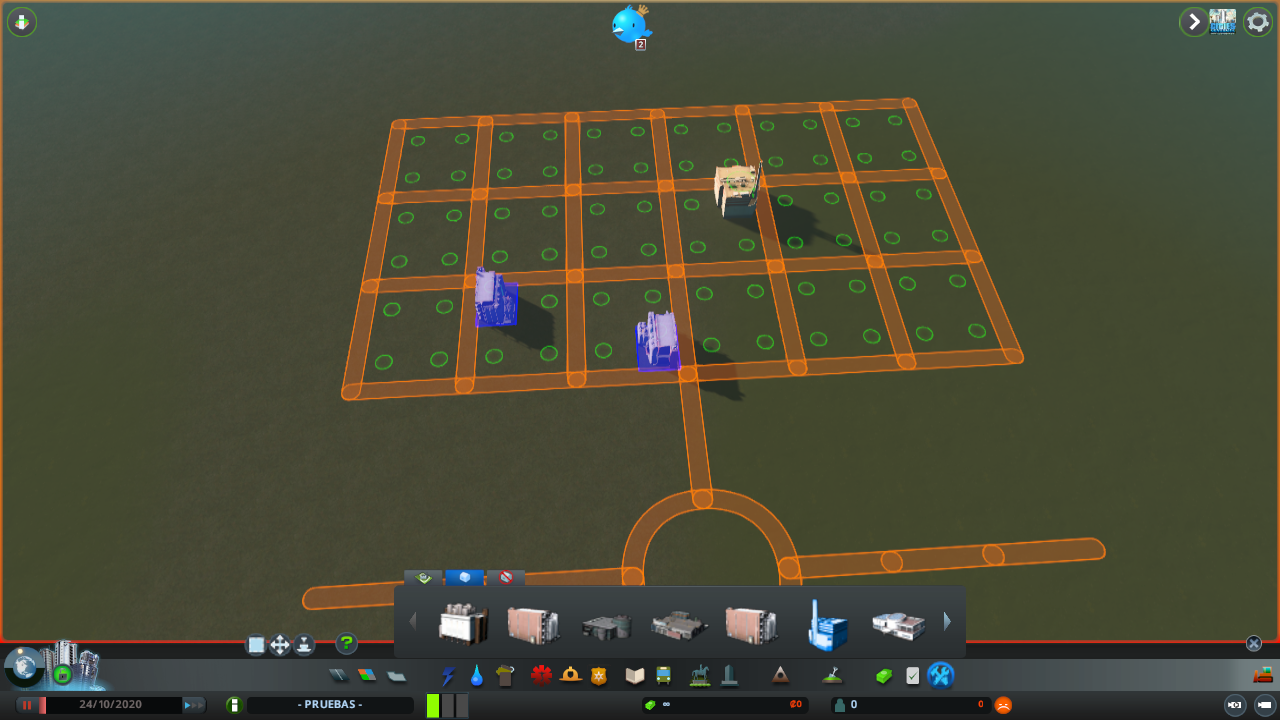
\includegraphics[width=\textwidth]{images/preferences}
	\caption{Varias preferencias de edificios posicionadas en la selección hecha.}
	\label{fig:distributions-panel}
\end{figure}

Una vez seleccionado un edificio, IndustryLP pasará a la acción de añadir preferencia/restricción, y junto a la distribución de carreteras nos saldrán puntos verdes en donde fijar la posición del edificio. Cuando estemos modificando preferencias, los edificios ya establecidos se nos mostrarán junto con el área edificable en color azul. En el caso de que estemos modificando restricciones, nos aparecerán solo los edificios indicados como restricción. \\

Si por un casual queremos borrar una selección, tendremos que pulsar el botón derecho del ratón cerca de una posición dada. \\

Una cosa a tener en cuenta es que, si pusieramos un mismo edificio como restricción y preferencia, el programa no generaría ninguna solución. Esto es debido a que el sistema lógico no encuentra una solución que satifaga las dos reglas a la vez.

\subsection{Generación de industrias}

Cuando tengamos una distribución generada, y opcionalmente marcadas las preferencias y restricciones, se nos habilitará el icono de la acción de \textbf{Generar soluciones}. Si la activamos, se nos mostrará el diálogo de la Figura \ref{fig:dialog} con varias opciones para modificar.

\begin{figure}[h]
	\centering
	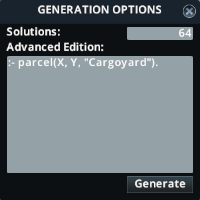
\includegraphics[width=0.5\textwidth]{images/dialog}
	\caption{Opciones de la generación.}
	\label{fig:dialog}
\end{figure}

\begin{enumerate}
    \item \textbf{Soluciones:} número de soluciones que el sistema deberá generar. 0 para generar todas las posibles.
    \item \textbf{Edición avanzada:} Nos permitirá incorporar reglas en el formato \textit{ASP Core 2}, que es el formato con el que trabaja la herramienta Clingo.
    
    Existen algunas reglas predefinidas de distancia y vecinos con las que podemos trabajar de forma inmediata. Otro tipo de reglas las deberemos escribir en este campo o crear un archivo de programa lógico, tal y como se expone en la Sección \ref{subsec:logic-files}.
\end{enumerate}

Si pulsamos en el botón \textbf{Generate}, el panel de opciones se nos modificará a como aparece en la Figura \ref{fig:solutions}. En esta nueva interfaz podremos destacar varias zonas:

\begin{figure}[h]
	\centering
	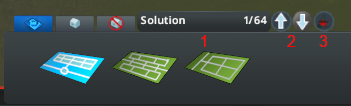
\includegraphics[width=\textwidth]{images/solutions}
	\caption{Menú de selección de solución.}
	\label{fig:solutions}
\end{figure}

\begin{enumerate}
    \item Panel con el índice de la solución actual / soluciones totales encontradas.
    \item Botones para ir a la solución anterior / posterior.
    \item Construir solución.
\end{enumerate}

El resultado de la generación de la solución actual se mostrará en la selección actualmente hecha. Cuando estemos convencidos con una solución, podemos pulsar el botón de construir solución y todo se construirá dentro de \cities.

\subsection{Edición avanzada}
\label{subsec:logic-files}

Otra opción para hacer una edición avanzada, y además de poder modificar la generación de IndustryLP con nuevas reglas es modificar los archivos con los programas lógicos que IndustryLP carga en cada generación. Si el mod ha sido instalado mediante Steam, estos archivos se localizarán en la ruta \texttt{Program Files (x86) / Steam / SteamApps / WorkShop / Content / 255710 / 2597556943 / logic\_program }. \\

Cualquier archivo que se cree en esta carpeta con la extensión \texttt{.lp} será cargado dentro del proceso de Clingo, por lo que el usuario puede crear archivos con programas lógicos a voluntad sin tener que recompilar el mod, y pudiendo persistir estos programas entre generación y generación.